\documentclass[letterpaper,11pt]{article}
\oddsidemargin -1.0cm \textwidth 17.5cm

\usepackage[utf8]{inputenc}
\usepackage[activeacute,spanish, es-lcroman]{babel}
\decimalpoint
\usepackage{amsfonts,setspace}
\usepackage{amsmath}
\usepackage{amssymb, amsmath, amsthm}
\usepackage{comment}
\usepackage{float}
\usepackage{amssymb}
\usepackage{dsfont}
\usepackage{anysize}
\usepackage{multicol}
\usepackage{enumerate}
\usepackage{graphicx}
\usepackage[left=1.5cm,top=2cm,right=1.5cm, bottom=1.7cm]{geometry}
\setlength\headheight{1.5em} 
\usepackage{fancyhdr}
\usepackage{multicol}
\usepackage{hyperref}
\usepackage{wrapfig}
\usepackage{subcaption}
\usepackage{siunitx}
\usepackage{cancel}
\usepackage{mdwlist}
\usepackage{svg}
\pagestyle{fancy}
\fancyhf{}
\renewcommand{\labelenumi}{\normalsize\bfseries P\arabic{enumi}.}
\renewcommand{\labelenumii}{\normalsize\bfseries (\alph{enumii})}
\renewcommand{\labelenumiii}{\normalsize\bfseries \roman{enumiii})}


\begin{document}

\fancyhead[L]{\itshape{Facultad de Ciencias F\'isicas y Matem\'aticas}}
\fancyhead[R]{\itshape{Universidad de Chile}}

\begin{minipage}{11.5cm}
    \begin{flushleft}
        \hspace*{-0.6cm}\textbf{FI1000-1 Introducción a la Física Clásica}\\
        \hspace*{-0.6cm}\textbf{Profesor:} Ignacio Bordeu\\
        \hspace*{-0.6cm}\textbf{Auxiliares:} Alejandro Cartes \& Simón Yáñez\\
        \hspace*{-0.6cm}\textbf{Ayudante:} Javier Cubillos\\
    \end{flushleft}
\end{minipage}

\begin{picture}(2,3)
    \put(366, 10){
\includegraphics[scale=0.9]{2020-1/Imágenes/logo/dfi-fcfm.pdf}}
\end{picture}

\begin{center}
	\LARGE\textbf{Auxiliar \#3}\\
	\Large{Movimiento Circular Uniforme}
\end{center}

\vspace{-1cm}
\begin{enumerate}\setlength{\itemsep}{0.4cm}

\rfoot[]{pág. \thepage}

\item[]

\item Considere una persona en la superficie de la Tierra a una latitud $\lambda$. Sabiendo que el radio de la Tierra mide $R_{\oplus}=\SI{6370}{\km}$ y su periodo de rotación es de $\SI{24}{\hour}$, determine: rapidez angular, rapidez tangencial y aceleración centrípeta. ¿Qué sucede en los polos y en el ecuador?

\item Dos tortugas comienzan una carrera desde el punto $A$. Una de ellas viaja en línea recta desde el punto $A$ hasta el punto $B$ con aceleración constante $a_0$, partiendo del reposo. La otra tortuga lo hace describiendo una semicircunferencia de radio $R$, moviéndose con rapidez constante. Si ambas llegan al mismo tiempo al punto $B$, ¿cuál es la velocidad angular $\omega$ de la segunda tortuga?
    
\begin{figure}[H]
    \centering
    \svgpath{../../2021-2/img/aux3}
    \hspace{1em}
    \begin{subfigure}[t]{0.35\textwidth}
        \centering
        \includesvg[width=1\linewidth]{carrera.svg}
    \end{subfigure}
\end{figure}

\begin{multicols}{2}
\item Un anillo muy pequeño se hace girar con velocidad angular constante $\omega$ a lo largo de una circunferencia vertical de radio $R$. La circunferencia está cortada en un punto determinado por un ángulo $\theta$, como se señala en la figura. Al alcanzar este punto, el anillo se desprende y continua en caída libre.

    \begin{enumerate}
        \item Calcule el valor de la velocidad angular $\omega$ si el anillo, luego de desprenderse, toca a la circunferencia en el punto $P$ (ver figura)
    
        \item Para el caso anterior indique la velocidad y la rapidez del anillo cuando cruza el diámetro de la circunferencia (eje $x$)
    \end{enumerate}
    \columnbreak
    \begin{figure}[H]
        \centering
        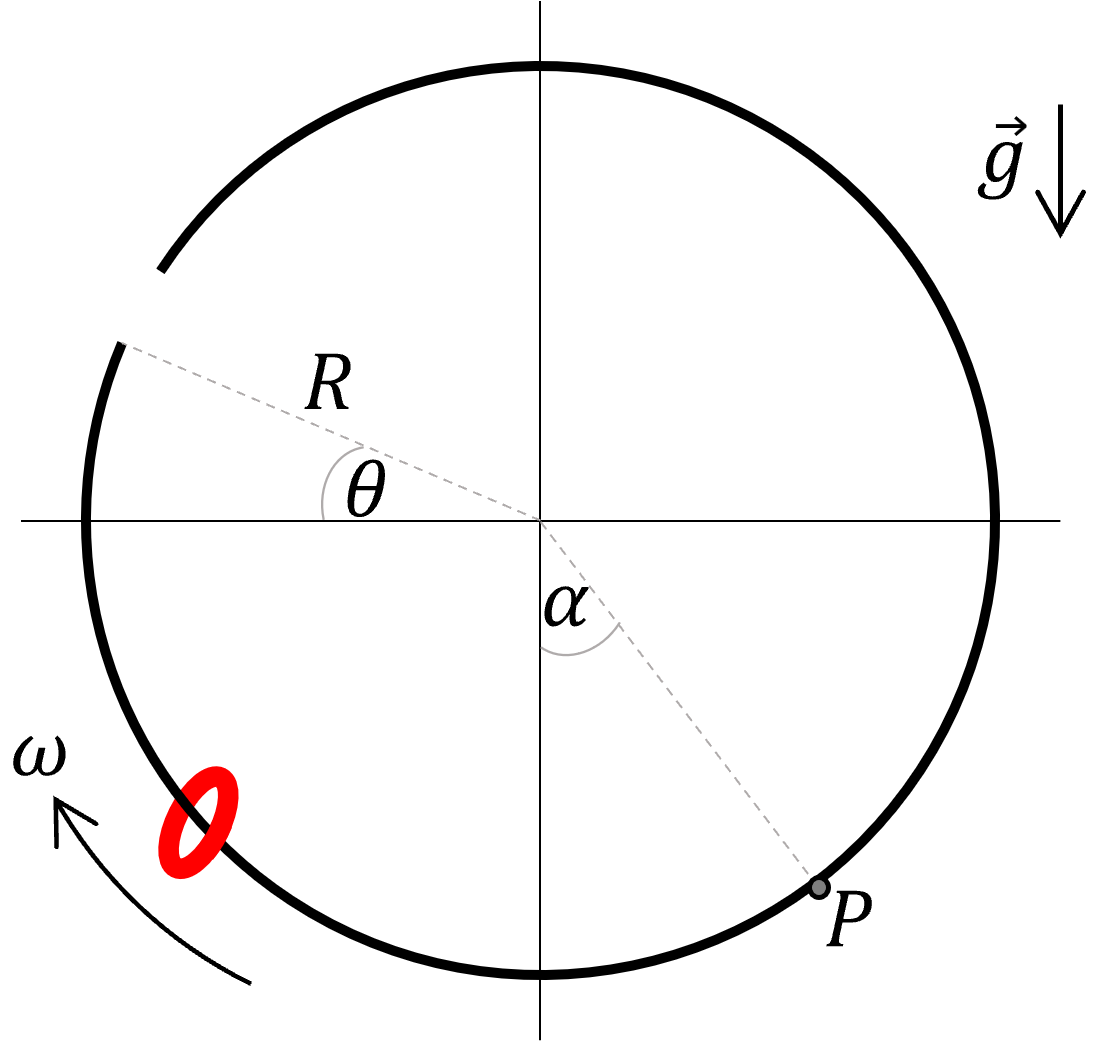
\includegraphics[scale = 0.7]{2023-1/img/aux_3/anillo.png}
    \end{figure}
\end{multicols}


% Para imágenes vectoriales -> el texto tiene que estar en LaTeX
% \begin{figure}[htbp]
%   \centering
%   \svgpath{../Imagenes/ejercicios}  -> .. irse pa'trás 
%   \includesvg{ej5.svg}
% \end{figure}

\end{enumerate}
\end{document}
